
\section{Multilayer Network}

In this section, the analysis will dive into all the unexplored paths, starting from Falkenberg’s work. In particular, the same polarization analysis will be conducted on a topic level: instead of computing it at a full network level, a retweet network was created for each topic, so the topics that were driving the polarization of cop emerged. Furthermore, the aim was also  to explore how the polarization of topics evolved over time.

By reading the previous section, the concept of topic modeling is known, and so is the way the main models perform. The goal is to create a multilayer network where every layer represents a topic.

In order to do so, a Python library was developed, which can be used as a toolbox, starting from the tweets fresh out from the official API of Twitter. The design is modular and can achieve different goals. In fact, even if the  interest is only in the retweet network of the users (nodes are users, ties are retweets), this framework can be used to perform different tasks, but to the purpose of this study the tasks highlighted are: 

\begin{itemize}
    \item Clustering tweets according to their topic
    \item Giving a meaningful label to the clusters
    \item Creating the retweet network (global and multilayer version)


\end{itemize}

The steps are independent, so, for example, it is possible to create the network without the need to run the topic modeling part.


\paragraph{Steps}
Even though some steps are avoidable, the natural and minimal pipeline follows these steps:


\begin{enumerate}
    \item from JSON to a tabular format 
    \item label each tweet with a topic
    \item create multilayer retweet network  
    
\end{enumerate} 


\subsection{Process input}

The first step consists of the transformation of the JSON objects into tabular data to optimize the space and handle the data in an easier way with pandas. This is also helpful to save space; in the case of COP26, a shift is made from a 14 GB JSON to a less than 2 GB CSV, since most of the fields are not relevant to this study.

In this process, all the tweets with attachments and not in English are discarded. The tweets are divided into multiple dataframes: one for original tweets - i.e., the ones that the author actively writes-, and one for the retweets.

At the end of this stage, a CSV and pkl file are saved in case somebody needs the tweets in tabular data. If the script is re-run and these files exist, they will be loaded instead of running the process again.


\subsection{Topic modeling}

As extensively discussed in chapter 2, in this segment of the pipeline the tweets can be labeled using Bertopic, with the possibility to choose the embedder; the one used in this research is\textit{ all-MiniLM-L6-v2}, the one evaluated in the previous section.

This step is the most computationally expensive; for this reason, to avoid redundancy, the topic modeling has been run only using original tweets.


After this step, all the original tweets are labeled with a numeric topic, and then the label has been propagated to all the retweets so that the entire dataset is now labeled with a topic.

At this point, the OpenAI API can be used to give a meaningful label to the topics, while beforehand, the labels were just made of the most relatively frequent words of the topic. By using the langchain library, it is possible to structure an employable  prompt. The model was assigned the words identified with TF-IDF and 3 representative tweets sampling a subset of the documents in each topic, and calculated on the cosine similarity between TF-IDF representations.


This is the one used: 
\\

\textit{    I want you to act as a tweet labeler, you are given representative words
from a topic and three representative tweets, give more attention to the words, all the tweets are related to climate change and COP, there is no need to mention them, detect subtopics.
start with "label:" and avoid hashtags,
which is a good short label for the topic containing the words [{words}]?, here are 3 tweets to help you:
first = "{tweet1}", second = "{tweet2}", third = "{tweet3}}
\\

Similarly to the previous stage, the labeled dataset is saved in the cache folder both in CSV and pkl. The model and the labels are saved, too.



\subsection{Network}
In this phase, after labeling the tweets, a retweet network will be created for each topic, gathering it all together in a multilayer network.
%The network is directed, the nodes are the users, and the tie is the number of retweets. For each topic, a network is created.

In the process of the creation of the network, there are retweeted tweets that do not have the original one, so they are  discarded.

The last step is the creation of a multilayer network using the multinet library developed by Uppsala University; Every layer is a retweet network of a specific topic. It was built starting from the subset of tweets of a specific topic, the unique users are the nodes and, if user A retweets user B there will be a tie $A \rightarrow B$. The network is directed and weighted with the number of retweets. Fig \ref{fig:multilayer} is a simple example of a network with 2 layers.

The network then has been filtered by removing the outlier layer, labeled with -1.

\paragraph{COP26 network}
For COP26, 70 layers were detected, the average number of users per layer is 8127, min is 15, max is 108829,

\paragraph{COP21 Network}
For COP26, 36 layers were detected, the average number of users per layer is 10123, min is 696, max is 142062,



\begin{figure}
    \centering
    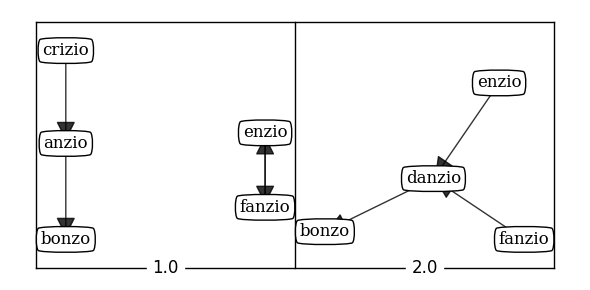
\includegraphics[width=0.75\linewidth]{Chapter4/figures/projected_topics_ml.png}
    \caption{Example of multilayer retweet network }
    \label{fig:multilayer}
\end{figure}




\section{Polarization}
At this point, for each layer, it is possible to compute for each user a latent ideology score, and then, using Hartigan’s diptest, a polarization value  can be assigned to each topic. More details on how this is computed are dealt with in the related works. In this process, there are some parameters that can be adjusted: the number of influencers - defined as the most retweeted users-, and $n$ - representing the minimum number of retweets a user should have made to an influencer to be considered-.

The ideology score is not computed on all the users, but when selecting the influencers, the users are limited to the ones that retweeted at least n times those influencers.

In order to have enough data to be analyzed, the values set were $n\_influencers = 100$ and $n=2$. The hartigan diptest requires a minimum of nodes to be statistically significant and, since at this point the layer are filtered, all the layers with a p-value of the diptest higher than 0.05 have been discarded.


\paragraph{COP26 }
The number of networks goes from 70 to 30 . The total influencers considered in the analysis of COP26 is 1698. 22302 users have an assigned score for cop26, with an average of 1311 actors per topic, with a min of 151 and a max of 7764.

\paragraph{COP21}
the number of networks went from 36 to 8. The total number of influencers considered in the analysis of COP21 is 392. 8020 users have an assigned score, with an average of 2058 actors per topic, with a min of 35 and a max of 7524. 

Tab  \ref{tab:recap_ideology} presents a summary of the starting networks 


\begin{table}[h]
    \centering
    \begin{tabular}{|l|l|l|l|}
        \hline
        \textbf{Description} & \textbf{COP21} & \textbf{COP26} & \textbf{COP2x}\\ \hline
        Initial topics & 36 & 70 & 54 \\ \hline
        Final topics & 8 & 26 & 29\\ \hline
        Influencers scored & 392 & 1557 & 1559\\ \hline
        Users scored & 8020 & 22161& 33312 \\ \hline
        Mean users/topic &  2058 & 1311 & 1766\\ \hline
        Min users/topic & 35 & 151 & 123\\ \hline
        Max users/topic & 7524 & 7764 & 14504\\ \hline
        diptest &1 & 0.07 & 0.05 \\ \hline
        \end{tabular}
        \caption{Summary of Latent ideology}
    \label{tab:recap_ideology}
\end{table}


\section{Logitudinal analysis}
In order to see topic polarization over time, we need to run the topic modeling with all the tweets. Still, there are too many, so instead of taking the original tweets of COP21 and COP26, we only take the original with at least one retweet which are around 1/3 of the total but are the one needed to create  the rest of the network.

Then the two dataset have been merged, we will refer to this dataset $COP2x$ and the same process described below has been done.




 
